\section{Causal Inference}
Given a \textbf{treatment}, we want to know if there is a \textbf{causality} between the \textbf{treatment and outcome}.

Given a \textbf{control group} and \textbf{treatment group}, if we can observe the before and after treatment for both groups, we can find out different treatment effects:
\begin{itemize}
	\item individual treatment effect: $Y_{1i} - Y_{0i}$
	\item average treatment effect: $E(Y_{1i} - Y_{0i})$
	\item subgroup treatment effect: $E(Y_{1i} - Y_{0i} | X)$
\end{itemize}
However, $Y_{1i}$ and $Y_{0i})$ can't be both observable for one group.

$\rightarrow$ approximation

\subsection{Data Collection in Causal Inference}
\paragraph{Golden Rule} \textbf{randomized controlled trials}. The treatment is controlled, individuals are assigned randomly to the treatment. 

$\rightarrow$ Sample selection bias is prevented.

\subsubsection{Different Types of Experiments/Data Collections}
\begin{itemize}
	\item \textbf{Randomized Controlled Trials}: Treatment/Control groups separated. Subject is \textbf{randomly assigned} to the \textbf{treatment/control} group.
	
	$\rightarrow$ minimum selection bias
	\begin{itemize}
		\item Lab Experiments
		\item Field Experiments
	\end{itemize}
	
	\item \textbf{Quasi-experiements}: \textbf{natural groups} pre-exist, no separation of control/treatment group beforehand. The independent variable(treatment variable) is \textbf{controlled}, subjects are \textbf{not randomly assigned}.
	
	$\rightarrow$ selection bias
	
	\item \textbf{Observational studies}: what we always have. The independent variable is \textbf{not controlled}, individuals \textbf{self-assigned}.
	
	$\rightarrow$ selection bias 
	\begin{itemize}
		\item cross-sectional study
		\item longitudinal study
		\item panel study
		\item case-control study
	\end{itemize}
\end{itemize}

\subsection{Challenges to Quasi-Experiments \& Observational Studies: Confounding Variables \& Identification Strategies}
\subsubsection{Confounding Variables}

 For \textbf{Quasi-Experiments and Observational Studies}, confounding variables might exist, but \textbf{not observable, therefore omitted from the model}. In order to identify precise causal effects, we need to deal with confounding variables.


\paragraph{Confounding Variables} an extraneous variable that is \textbf{unobservable}, which \textbf{correlates} with \textbf{dependent and independent variables}.

$\rightarrow$ $Cov(\varepsilon, X) \neq 0$ $\rightarrow$ Endogeneity

$\rightarrow$ Consequence: biased results.

\subsubsection{Combat Confounding Variables by Data Collection: Randomized Controlled Trials}
Apply Randomized Controlled Trials: confounding variables \textbf{automatically removed}.

Ways to conduct RCTs:
\begin{itemize}
	\item Lab experiment
	\item Field experiement
\end{itemize}
\begin{figure}[H]
	\centering
	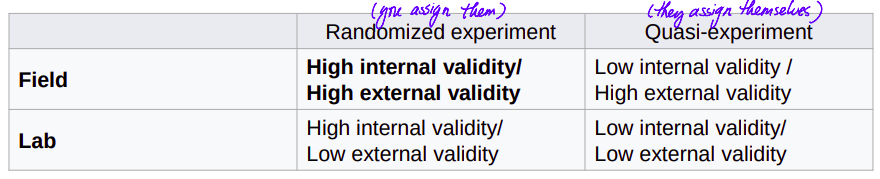
\includegraphics[width=0.8\textwidth]{labfield.png}
\end{figure}
\subsubsection{Indentification Strategy for Quasi-Experiments: Difference-in-Difference}
\begin{itemize}
	\item Idea: Observe the \textbf{effect of treatment} controlled by the researcher between \textbf{control \& treatment group}, \textbf{over time}. 
	\item Process:
	\begin{itemize}
		\item Assume there exists an \textbf{overall trend} on both control \& treatment group. We still want to estimate the treatment effect while not omitting confounding variable (eg: time). 
		\item treatment effect:
		$$\text{Treatment effect} = (Y_{t2} - Y_{t1}) - (Y_{c2} - Y_{c1})$$
	\end{itemize}
\end{itemize}




\subsubsection{Indentification Strategy for Panel Studies: Fixed-Effect Models}
\begin{itemize}
	\item Idea: \textbf{Fixed influence} is omitted as one of the confounding variables in modeling the treatment effect on outcome.
	
	$\rightarrow$ model \textbf{fixed effect} to soak up \textbf{individual effects on model}.
	\item Fixed-Effect Model: the fixed effect is modeled as an \textbf{additional intercept $\lambda_i$} for \textbf{each individual}.
\end{itemize}

\subsubsection{Indentification Strategy for Observational Studies: Propensity Score Matching}
\begin{itemize}
	\item Idea: in cross-sectional data, find a \textbf{data section} where control \& treatment group has the \textbf{maximum similarity} in covariate distribution. 
	
	$\rightarrow$ resembles \textbf{randomized experiment}
	
	\item Process:
	\begin{itemize}
		\item estimate \textbf{propensity score} by logistic regression for each individual in \textbf{treatment group}. 
		\item \textbf{match} the \textbf{control group} to the treatment group. Find subjects with \textbf{similar propensity score}.
		\item evaluate quality of matching
		\item evaluate \textbf{treatment effect} based on the \textbf{treatment and matched control group}.
		
	\end{itemize}
\end{itemize}

\subsubsection{Confounding Variable as Instrument Variables}
\paragraph{Instrument} attributes that \textbf{has causal effect} on \textbf{treatment variable}, but \textbf{no causal effect} on \textbf{outcome}.
\begin{itemize}
	\item Modeling Process:
	\begin{itemize}
		\item instruments \textbf{randomly assigned} to the treatment variable
		\item model the relationship between the instrument and treatment variable.
		\item model the relationship between the predicted treatment variable and outcome.
	\end{itemize}
	\item Estimation: 2-stage least square.                                                                                                                                                                                   
\end{itemize}

